\documentclass[a4paper, 10pt]{article}
\usepackage[utf8]{inputenc}
\usepackage[T1]{fontenc}
\usepackage[scale=.84]{geometry}
\usepackage[french]{babel}
\usepackage{hyperref}
\usepackage{graphicx}
\usepackage{amsmath}
\usepackage{amssymb}
\usepackage{minted}

\title{Réseaux\\Projet : tunnel IPv6-IPv4}
\author{Manon GIRARD - Enzo CADONI}
\date{}

\begin{document}
  \maketitle
  \newpage
  \tableofcontents
  \newpage

  \section*{Introduction}
    On se propose de réaliser un tunnel permettant à deux LAN IPv6 de
    communiquer de manière bidirectionnelle par le biais d'un ou plusieurs LAN
    IPv4. Le tunnel aura donc pour but de se positionner sur une machine pouvant
    communiquer avec les deux types de LAN et ainsi permettre la communication.
    Afin de pouvoir transmettre le traffic IPv6 par des LAN IPv4, le tunnel
    encapsulera le traffic IPv6 dans des paquets TCP/IPv4. \\

    Le langage choisi pour programmer ce tunnel est le langage C. En effet, ce
    langage permet de pouvoir observer en détail le fonctionnement des objets
    que l'on utilise, notamment les appels système. Aussi, C permet de
    programmer de manière modulaire plus clairement qu'avec Python.

  \section{Configuration réseaux}
    \subsection{Topologie et Adressage}
      Nous disposons d'un réseau de 6 machines virtuelles (VM), \verb+VM1+,
      \verb+VM2+ et \verb+VM3+ peuvent communiquer par IPv4 entre elles, tout
      comme \verb+VM1+, \verb+VM1-6+, \verb+VM2-6+, \verb+VM3-6+ et \verb+VM3+
      le peuvent par IPv6.

      Les VMs disposent toutes d'un fichier de configuration ansible situé dans
      leur répertoire. On pourra le retrouver dans le système de fichier interne
      des VMs dans le répertoire \verb+/vagrant/+. \\


    \subsection{Un grand malheur !}
      Afin de simuler la perte de \verb+VM2-6+, on enlève la machine du réseau
      et on supprime tout ce qui est superflu sur les autres machines, c'est à
      dire les interfaces et les routages qui étaietn nécessaires à \verb+VM1-6+
      et à \verb+VM3-6+ pour communiquer avec elle. Il ne reste donc à ces deux
      machines qu'une interface dotée d'une IPv6. \\

      Il faut désormais construire un tunnel afin que VM1-6 et VM3-6 puissent à
      nouveau communiquer.

  \section{L'interface virtuelle TUN}
    Afin de manipuler des interfaces virtuelles TUN, on crée la bibliothèque
    \verb+iftun+.

    \subsection{Création de l'interface}
      Afin de pouvoir créer une interface TUN, une fonction \verb+tunalloc+ est
      rajoutée à la bibliothèque \verb+iftun+.

      On remarque que l'interface (ici tun0) créé en utilisant \verb+tunalloc+
      n'est pas persistente lorsque le programme l'interface termine, il faut
      donc pouvoir la créer, la configurer et l'utiliser avant que le programme
      qui l'ai créé ne termine.

      \verb+tunalloc+ aura aussi pour but de renvoyer le descripteur de fichier
      correspondant à l'interface. \\

    \subsection{Configuration de l'interface}
      Dans le but de configurer tun0 après sa création et avant que le programme
      ne commence à l'utliser, nous allons créer un script bash permettant à
      \verb+tun0+ de s'activer et de posséder une adresse IPv6, en l'occurence
      \verb+fc00:1234:ffff::1+. \\

      Ce script est donc pour l'instant composé des deux commandes suivantes
      \begin{verbatim}
        # Activation de tun0 dans le cas ou elle serait inactive
        ip link set tun0 up

        # Ajout d'une IPv6 à tun0
        ip -6 a add fc00:1234:ffff::32 dev tun0
      \end{verbatim}

      On affecte le masque /32 à \verb+tun0+ afin que les adresses IPv6 des
      différents LAN soient reconnues comme faisant partie du sous-réseau de
      \verb+tun0+, les paquets passeront donc par le tunnel sans routage
      supplémentaire sur la machine créant \verb+tun0+.

      Lorsqu'on réalise un ping sur l'adresse IP de l'interface \verb+tun0+ à
      savoir \verb+fc00:1234:ffff::1+, on peut observer qu'aucun paquet n'est
      intercepté par \verb+wireshark+ sur tun0, mais que le ping obtient une
      réponse depuis la machine où on le réalise. \\

      En revanche, lorsqu'on réalise un ping sur une adresse telle que
      \verb+fc00:1234:ffff::10+, qui ne correspond à aucune machine mais faisant
      partie du sous-réseau de \verb+tun0+, \verb+wireshark+ intercepte les
      paquets en destination de l'adresse sur \verb+tun0+. On peut observer une
      capture d'un ping sur cette adresse dans le fichier
      \verb+captures/ping_tun0:10.pcapng+.\\

      Une explication pourrait etre la suivante, l'interface \verb+tun0+ ne
      traite pas les paquets qui ont pour destination l'interface elle meme,
      elle peut néanmoins renvoyer une réponse si le paquet en exige une, par
      exemple dans le cas d'un paquet ICMP envoyé durant un ping.
      Lorsqu'on réalise un ping sur une adresse présente dans le sous-réseau de
      \verb+tun0+, à savoir \verb+fc00:1234::/32+, \verb+tun0+ transmet les
      paquets, et donc les traite, ils sont donc visible sur \verb+tun0+ depuis
      \verb+wireshark+

    \subsection{Récupération des paquets}

      L'interface \verb+tun0+ est créée, on dispose maintenant d'un descripteur
      de fichier lui correspondant permettant de lire des informations. On crée
      une fonction \verb+transfert+ dans le bibliothèque \verb+iftun+, ayant
      pour but d'écrire d'un fichier \verb+src+ dans un fichier \verb+dest+.

      Nous allons nous servir de la fonction transfert afin de rediriger des
      flux vers \verb+tun0+ et inversement. \\

      On peut imprimer le flux de \verb+tun0+ sur la sortie standard en
      utilisant la fonction de transfert (la source est le descripteur de
      fichier de \verb+tun0+, la destination est le descripteur de la sortie
      standard, soit 1). On filtrera la sortie grace à \verb+hexdump+ afin de ne
      pas essayer d'imprimer des caractères non imprimables. On peut voir dans
      le fichier \verb+captures/sortie_test_iftun.log+ un exemple de redirection
      du flux de \verb+tun0+ sur la sortie standard (filtré par \verb+hexdump+).

      On peut observer que rien n'est imprimé lorsque l'on réalise un ping
      \verb+fc00:1234:ffff::1+ et que le traffic IPv6 transféré par \verb+tun0+
      est imprimé lorsqu'on réalise un ping sur \verb+fc00:1234:ffff::10+.
      L'hypothèse permettant d'expliquer ce résultat est la meme que celle
      permettant d'expliquer pourquoi \verb+wireshark+ intercepte ou non les
      paquets envoyés durant ces pings. \\

      Le fichier \verb+captures/sortie_test_iftun.log+ correpond à la capture
      \verb+captures/ping_tun0:10.pcapng+ déjà observée précedemment. On peut
      observer que les paquets (en vue héxadécimale) correspondent à ce que l'on
      peut voir d'imprimé sur la sortie standard (dans le log). \\

      Enfin, l'option \verb+IFF_NO_PI+ permet de se passer des 4 octets
      précedents les paquets reçus par l'interface étant composés de 2 bits
      octets de flags et de deux autres renseignant le protocole utilisé.

      Si l'on ajoute cette option, on diminuera donc le nombre d'octet lu et
      écrit dans la fonction de transfert.

  \section{Un tunnel simple pour IPv6}
    Nous allons ici construire pas à pas le tunnel bidirectionnel qui permettra
    aux deux LAN (3 et 4) séparées de pouvoir à nouveau communiquer.

    \subsection{Redirection du trafic entrant}
      Dans le but de pouvoir gérer le traffic entre les extrémités du tunnel,
      nous allons créer la bibliothèque \verb+extremite+, elle contiendra deux
      fonctions, \verb+ext_out+ et \verb+ext_in+ \\

      \verb+ext_out+ aura pour but, dans un premier temps, de créer un serveur
      via une socket. Ce serveur aura pour but d'écouter sur le port 123 et de
      rediriger le traffic sur la sortie standard.

      \verb+ext_in+ devra se connecter via une connexion TCP au serveur qu'a
      ouvert l'autre extrémité du tunnel sur le meme port. La fonction devra
      ensuite transmettre le traffic lu sur \verb+tun0+ sur la socket. \\

      En lisant le manuel des appels système \verb+recv+ et \verb+send+
      permettant de lire et d'écrire avec une socket, on observe que ces appels
      sont respectivement équivalents aux appels système \verb+read+ et
      \verb+write+ si l'option \verb+flags+ de ces appels est égal à 0, c'est à
      dire que nous n'avons pas besoin d'options particulière. Nous n'avons
      besoin d'aucune option, nous pouvons donc utiliser la fonction
      \verb+transfert+ de la bibliothèque \verb+iftun+ pour transferer un flux
      vers la socket ou inversement. \\

      On déploie un programme exécutant \verb+ext_in+ sur VM1 et un autre
      exécutant \verb+ext_out+ sur VM3, on ping ensuite \verb+fc00:1234:ffff:10+
      sur VM1 afin d'injecter du traffic dans l'interface \verb+tun0+ de VM1. \\

      On peut tester le déploiement en se plaçant au niveau de \verb+VM2+ sur
      \verb+wireshark+ et en faisant un ping de \verb+VM3-6+ depuis
      \verb+VM1-6+. On peut voir dans \verb+captures/sortie_test_ext.log+ la
      sortie standard de \verb+VM3+ une fois \verb+ext_out+ lancée. En comparant
      le log à la capture \verb+captures/test_ext_VM2.pcapng+ et
      particulièrement la section données des paquets TCP émis par
      \verb+172.16.2.131+, on voit que les paquets contiennent bien le
      datagramme IPv6 encapsulé au niveau de \verb+VM1+.

    \subsection{Redirection du trafic sortant}
      Afin de pouvoir transmettre le traffic sortant par \verb+ext_out+ sur
      l'interface \verb+tun0+ locale, au lieu de rediriger le traffic sur
      l'entrée standard, on le redirige directement dans \verb+tun0+ dans
      \verb+ext_out+.

      Cette modification permettra au datagramme IPv6 conduit par le tunnel
      d'etre transmis par \verb+tun0+ vers sa destination. En effet, lorsque
      l'on écrit dans le fichier correspondant à \verb+tun0+, l'interface
      interprète les paquets comme si ils étaient envoyés par une machine (par
      exemple par un ping), \verb+tun0+ se charge donc de les retransmettre. \\

      On lance \verb+ext_in+ sur \verb+VM1+, \verb+ext_out+ sur \verb+VM3+ puis
      on capture dans le fichier \verb+captures/test_tun0_ext_out.pcapng+ sur
      l'interface \verb+tun0+ les paquets envoyés par \verb+VM1-6+ à
      \verb+VM3-6+. On extrait un paquet en hexadécimal (ASCII dans un premier
      temps) dans le fichier \verb+captures/paquet_tun0_VM3.hexdump+, on peut
      aisément voir dans ce paquet les adresses sources et destination,
      respectivement les adresses de \verb+VM1-6+ et de \verb+VM3-6+. Ce paquet
      est un paquet \verb+ICMPv6+ comme on pouvait s'y attendre. \\

      On peut injecter ce paquet manuellement dans tun0 (grâce à \verb+netcat+
      par exemple), cela aura le même effet que de l'injecter directement à
      partir du client comme le fait la fonction \verb+ext_out+ en l'état
      actuel. Il faut faire en revanche faire attention à maintenir à jour le
      CRC du datagramme si on souhaite le modifier, sinon, il y a une très forte
      probabilité pour que le paquet soit considéré comme corrompu. Le CRC peut
      être recalculé en faisant le complément à 1 de la somme des compléments à
      1 des valeurs des octets du paquet et doit être exprimé sur deux octets.

    \subsection{Intégration Finale du Tunnel}
      Nous avons désormais la possibilité de réaliser un tunnel unidirectionnel
      en lançant \verb+ext_in+ sur une extrémité de tunnel et \verb+ext_out+ sur
      l'autre. Pour assurer la bidirectionnalité du tunnel, il faudra lancer les
      deux fonctions en meme temps, nous allons pour cela utiliser des threads
      POSIX (\verb+pthreads+). \\

      les deux fonctions (\verb+ext_in+, \verb+ext_out+) seront chacune lancées
      dans un thread, il y aura donc deux threads en plus du thread principal.

      le programme ainsi lancé sur les deux extrémités, ces dernières pourront
      communiquer de manière bidirectionnelle. \\

      On peux vérifier que les communications en réaliant un ping depuis deux
      terminaux différents sur VM3, on voit que les réponses arrivent
      alternativement sur les deux terminaux, les communications sont donc bien
      asynchrones.

    \newpage
    \subsection{Mise en place du tunnel entre VM1 et VM3 : Schémas}
      Ici un schéma détaillé du traffic passant par le tunnel sur une extrémité
      de ce dernier.

      \begin{figure}[h]
        \centering
        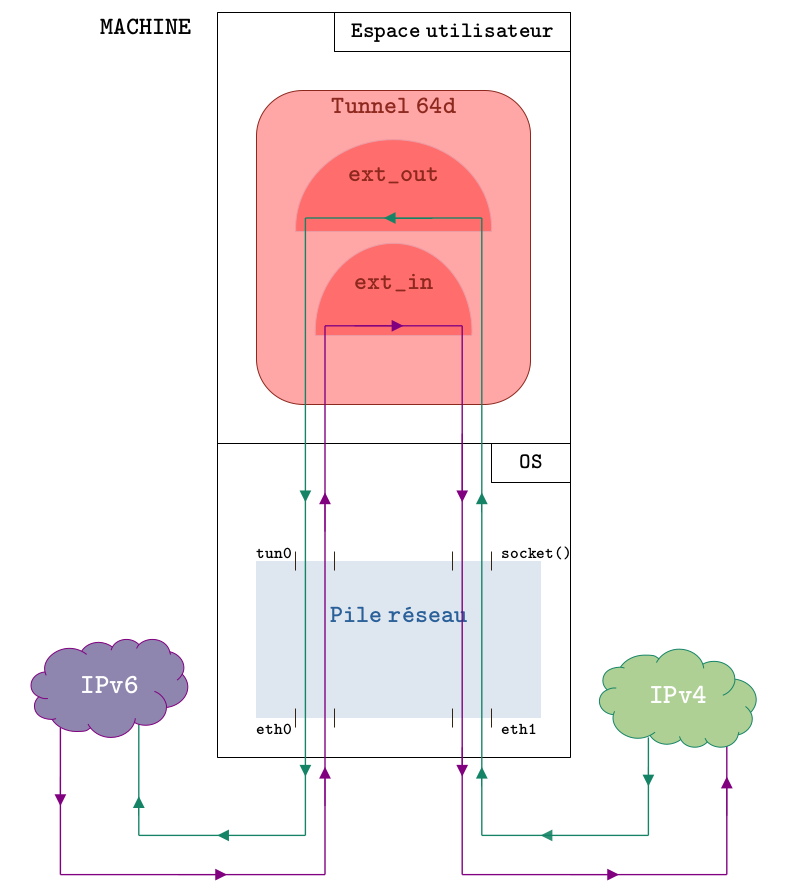
\includegraphics[scale=0.44]{img/schema_tunnel.png}
        \caption{Schéma d'un tunnel IPv6 vers IPv4}
      \end{figure}

      On peut voir ici un schéma plus détaillé du comportement du tunnel dans le
      réseau de 6 VMs que l'on manipule et de l'encapsulation des paquets.

      \begin{figure}[h]
        \centering
        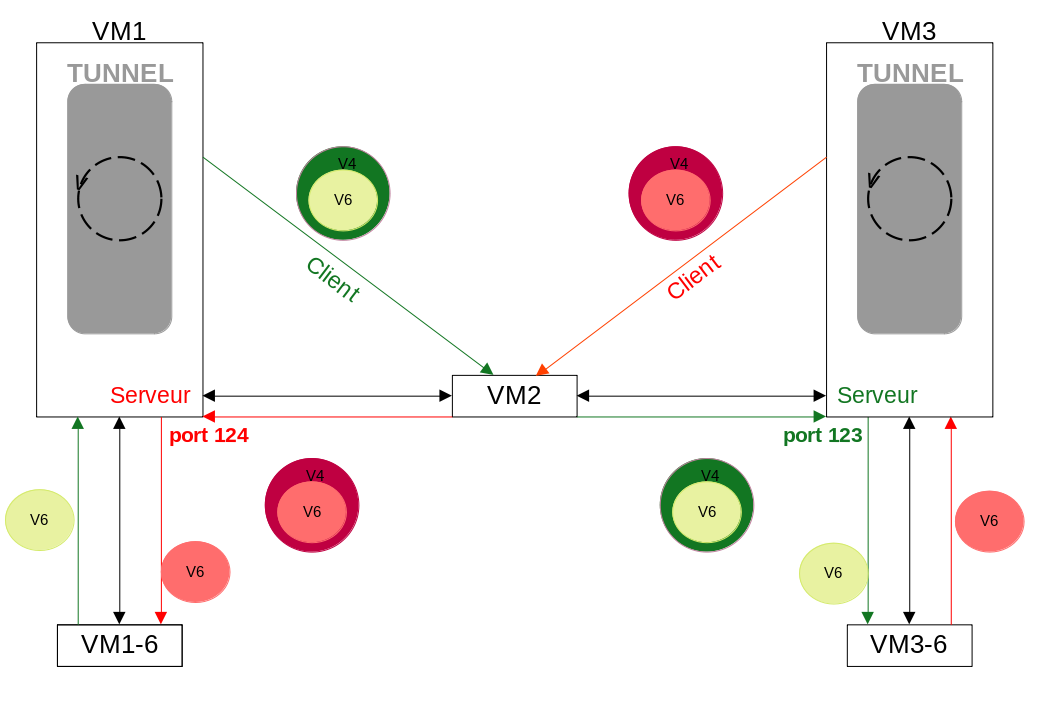
\includegraphics[scale=0.44]{img/explication.png}
        \caption{Comportement du tunnel et encapsulation}
      \end{figure}

    \newpage
    \subsection{Mise en place du tunnel entre VM1 et VM3 : Système}
      Nous avons enfin un exécutable permettant de lancer le tunnel
      bidirectionnel sur une machine, nommé \verb+tunnel64d+. \\

      Cet exécutable prendra sa configuration dans un fichier \verb+tunnel.conf+
      qui devra etre situé dans le répertoire \verb+/vagrant+ de la machine. Ce
      fichier devra etre de la forme :
      \begin{verbatim}
        ...
        dev=
        ...
        portin=
        ...
        portout=
        ...
        ipout=
        ...
      \end{verbatim}

      \begin{itemize}
        \item \verb+dev+ doit etre égal à l'interface TUN que le tunnel va
              devoir utiliser (après l'avoir créée), exemple : \verb+tun0+.
        \item \verb+portin+ doit etre égal au port par lequel on souhaite écrire
              les données transitant par l'interface.
        \item \verb+portout+ doit etre égal au port sur lequel on souhaite
              écouter les données émises par l'autre extrémité du tunnel.
        \item \verb+ipout+ doit etre égal à l'IPv4 de l'autre extrémité du
              tunnel
        \item \verb+...+ peut représenter tout texte superflu, dont d'éventuels
              commentaires \\
      \end{itemize}

      On peut voir en lancant le tunnel sur les deux extrémités que les machines
      peuvent se voir sur le réseau, on peut lancer un ping d'une machine vers
      l'autre et observer que le ping reçoit une réponse, le tunnel est donc
      bien bidirectionnel.

  \section{Validation Fonctionnelle}
    \subsection{Configuration}
      Le tunnel est en place sur les machines \verb+VM1+ et \verb+VM3+, en
      respectant l'architecture réseau vue précédemment. Les paramètres réseaux
      significatifs sur les machines lorsque le tunnel est actif sur le réseau
      sont :

      \begin{itemize}
        \item \verb-VM1-
              \begin{itemize}
                \item Adresses IP :
                      \begin{itemize}
                        \item \verb+eth1 : 172.16.2.131/28+
                        \item \verb+eth2 : fc00:1234:3::1/64+
                        \item \verb+tun0 : fc00:1234:ffff::1/32+
                      \end{itemize}

                \item Routes :
                      \begin{itemize}
                        \item \verb+172.16.2.160/28 via 172.16.2.132 dev eth1+
                      \end{itemize}
              \end{itemize}

        \item \verb+VM2+
              \begin{itemize}
                \item Adresses IP :
                      \begin{itemize}
                        \item \verb+eth1 : 172.16.2.132/28+
                        \item \verb+eth2 : 172.16.2.162/28+
                      \end{itemize}
              \end{itemize}

        \item \verb+VM3+
              \begin{itemize}
                \item Adresses IP :
                      \begin{itemize}
                        \item \verb+eth1 : 172.16.2.163/28+
                        \item \verb+eth2 : fc00:1234:4::3/64+
                        \item \verb+tun0 : fc00:1234:ffff::1/32+
                      \end{itemize}

                \item Routes :
                      \begin{itemize}
                        \item \verb+172.16.2.128/28 via 172.16.2.162 dev eth1+
                      \end{itemize}
              \end{itemize}

        \item \verb+VM1-6+
              \begin{itemize}
                \item Adresses IP :
                      \begin{itemize}
                        \item \verb+eth1 : fc00:1234:3::16/64+
                      \end{itemize}

                \item Routes :
                      \begin{itemize}
                        \item \verb+default via fc00:1234:3::1+
                      \end{itemize}
              \end{itemize}

        \item \verb+VM3-6+
              \begin{itemize}
                \item Adresses IP :
                      \begin{itemize}
                        \item \verb+eth1 : fc00:1234:4::36/64+
                      \end{itemize}

                \item Routes :
                      \begin{itemize}
                        \item \verb+default via fc00:1234:4::3+
                      \end{itemize}
              \end{itemize}
      \end{itemize}

    \subsection{Couche 3}
      Dans le but de vérifier que le tunnel est fonctionnel, on peut réaliser un
      ping de \verb+VM1-6+ depuis \verb+VM3-6+. On peut observer que le ping
      reçoit une réponse, le tunnel est donc fonctionnel. \\

      La capture \verb+captures/test_ping_tunnel_VM2.pcapng+ est ce que l'on
      peut observer au moment du ping sur \verb+VM2+ et la capture
      \verb+captures/test_ping_tunnel_VM3.pcapng+ est ce que l'on peut observer
      au moment du ping sur \verb+VM3-6+, la machine cible.

      On peut voir sur la capture de \verb+VM3-6+ que des paquets \verb+ICMPv6+
      arrivent bien sur la machine avec comme adresse source celle de
      \verb+VM1-6+ et que la machine lui répond avec d'autres paquets
      \verb+ICMPv6+. Aussi depuis VM2, on peut observer les requêtes et les
      réponses que se font \verb+VM1+ et \verb+VM3+. \\

      On pourrait aussi essayer de réaliser un ping depuis \verb+VM1+ vers
      \verb+VM3+ ou bien \verb+VM3-6+. On remarque dans un premier temps que
      cela ne fonctionne pas. En effet, en regardant sur wireshark, on peut voir
      que la source du paquet \verb+ICMPv6+ est l'adresse IP de \verb+tun0+, la
      réponse du ping arrive donc sur cette meme adresse IP et se trouve donc
      ignorée. \\

      Il est néanmoins possible de réaliser ce ping en précisant l'interface
      duquel on souhaite initialement lancer le ping, il suffit de rajouter
      l'option \verb+-I+ suivie de l'adresse IP de l'interface depuis laquelle
      on souhaite lancer le ping (exemple : la commande
      \verb+ping6 -I fc00:1234:3::1 fc00:1234:4::3+ permet de ping la machine
      \verb+VM3+ depuis \verb+VM1+ par le tunnel).

    \subsection{Couche 4}
      Afin de tester si il est possible d'utiliser le service \verb+echo+ de
      \verb+VM3-6+ depuis une machine du \verb+LAN3+, nous allons créer un
      fichier que nous allons envoyer grâce à \verb+netcat+. \\

      On met dans un fichier \verb+test.txt+ le message \verb+"test abcd 1234"+.
      Nous faisons une capture sur \verb+VM3-6+ au moment où l'on exécute la
      commande \verb+telnet fc00:1234:4::36 echo < test.txt+. On peut voir dans
      la capture \verb+captures/test_service_echo.pcapng+ que le message est
      bien reçu par \verb+VM3-6+ et que cette dernière répond.

    \subsection{Couche 4 : bande passante}
      L'utilitaire \verb+iperf3+ permet de réaliser divers tests sur les
      performances de connexion, nous allons l'utiliser pour tester la bande
      passante du tunnel.

      On teste le débit avec différentes tailles de tampon

      \begin{figure}[h]
        \centering
        \begin{tabular}{|c|c|}
          \hline
          taille du tampon & débit \\
          \hline
          10o & 2.98Kbits/sec \\
          2Ko & 610Kbits/sec \\
          128Ko & 2.99Mbits/sec \\
          1Mo & 3.39Mbits/sec \\
          \hline
        \end{tabular}
        \caption{Comparaisons de la bande passante du tunnel en fonction de la
        taille du tampon utilisée}
      \end{figure}

      On remarque que la bande passante augmente quand la taille du tampon
      augmente.

  \section{Améliorations}
    \subsection{Prise en compte de la taille des paquets}
      Afin d'alléger la lecture de l'extrémité finale du tunnel, on peut prendre
      en compte la taille des paquets y transitant. \\

      Tout d'abord, rappelons que l'appel système \verb+read+ renvoie le nombre
      d'octet qu'il a lu à partir du descrpteur de fichier qu'on lui a donné, on
      peut se servir de ce retour pour déterminer la taille d'un paquet dans
      \verb+ext_in+. Le nombre d'ocets à lire passé en paramètre de \verb+read+
      dans le transfert de \verb+ext_in+ sera égal au \verb+MTU+ de \verb+tun0+.

      Sachant que la taille d'un paquet peut être supérieure à 256, on va écrire
      la taille du paquet sur deux octets. On va ensuite envoyer ces deux octets
      avant d'écrire le paquet dans le tunnel. À la réception de cette entête,
      l'autre extrémité du tunnel (la fonction \verb+ext_out+) va pouvoir lire
      exactement le nombre d'octets que contient le paquet, puis l'écrire dans
      le \verb+tun0+ local. \\

      En terme d'implémentation, on passera un paramètre à la fonction existante
      \verb+transfert+ de la bibliothèque \verb+iftun+, selon si on est dans la
      fonction \verb+ext_out+, ou bien dans la fonction \verb+ext_in+. On peut
      voir l'impléntation finale de la fonction \verb+transfert+ dans le fichier
      \verb+src/iftun.c+.

    \subsection{Configuration ansible}
      On pourrait se demander si une configuration via \verb+ansible+ peut
      permettre de lancer le tunnel, la difficulté de cette tâche est de faire
      lancer un processus asynchone par \verb+ansible+. \\

      Tout d'abord, \verb+ansible+ est doté d'un module \verb+make+ qui permet
      d'exécuter la commande make dans le dossier choisis en spécifiant un champ
      \verb+chdir+, on ajoute donc les lignes suivantes aux configurations qui
      en auront besoin.

      \begin{minted}{yaml}
        - name: Compilation de l'utilitaire de lancement du tunnel
          make:
            chdir: /mnt/partage/tunnel64d
      \end{minted}

      Il est aussi possible de lancer une tache asynchrone dans \verb+ansible+ à
      l'aide des champs \verb+async+ et \verb+poll+, exemple :

      \begin{minted}{yaml}
        - name: ...
          shell: ...
          async: 50
          poll: 10
      \end{minted}

      \verb+async+ représente le nombre de secondes que laisse \verb+ansible+ à
      la tâche pour s'exécuter. \verb+poll+ représente l'intervalle de temps que
      va mettre \verb+ansible+ à revenir vérifier le statut de la tâche.

      La solution serait pour notre cas, avec une valeur 2628000 pour
      \verb+async+, l'équivalent d'un mois en secondes :

      \begin{minted}{yaml}
        - name: Lancement du tunnel
          shell: /mnt/partage/tunnel64d/bin/tunnel64d
          async: 2628000
          poll: 0
      \end{minted}

      L'inconvénient de cette option est qu'elle est limitée dans le temps, bien
      que nous puissions mettre l'équivalent d'un mois en secondes. Nous avons
      cherché une autre façon de procéder. \\

      La commande \verb+UNIX+ \verb+nohup+ permet de lancer un processus et le
      rendre persistent même si l'on ferme le terminal où la commande est
      appellée et même si l'utilisateur qui a exécuté le commande se déconnecte.

      On peut utiliser la commande comme suit dans la configuration
      \verb+ansible+ :

      \begin{minted}{yaml}
        - name: Lancement du tunnel
          shell: nohup /mnt/partage/tunnel64d/bin/tunnel64d
      \end{minted}

      Nous avons enfin remarqué quelque chose d'étrange, en effet, le programme
      lancé ne se ferme pas si la sortie standard et la sortie d'erreur du
      programme lancé ne sont pas redirigées, comme ceci :

      \begin{minted}{yaml}
        - name: Lancement du tunnel
          shell: nohup /mnt/partage/tunnel64d/bin/tunnel64d >/dev/null 2>&1 &
      \end{minted}

      Une autre particularité est le rajout d'un utltime \verb+&+ à la fin de la
      commande. Normalement, la seule utilisation de \verb+&+ en fin de commande
      permet de lancer en fond une tâche dépendante du terminal contrairement à
      \verb+nohup+. Nous observons qu'\verb+ansible+ bloque au lancement du
      programme et ne veux pas laisser la main au système sans que l'on ajoute
      ce \verb+&+.

      Quant aux redirections des sorties, nous pensons qu'ansible ne permet pas
      à \verb+nohup+ de lèguer la main au système tant que la sortie du
      programme continue d'imprimer, et le programme contient effectivement des
      appels à la fonction \verb+fprintf+ vers la sortie d'erreur.

      Nous allons donc utiliser cette manière de lancer le tunnel car non
      limitée dans le temps.

\end{document}
